\chapter{Qualitätssicherung}
\label{chap:Qualitätssicherung}
Die Qualität des Source-To-Source Compilers muss während und nach der erfolgreichen Implementierung sichergestellt werden. In diesem Kapitel werden im ersten Abschnitt die Komponententests als Qualitätsischerungsmaßnahme wärend der Entwicklung thematisiert.  Anschließend wird die Funktionsweise mithilfe einer speziell entwickelten Xamarin.Forms App überprüft.  Anhand dieses Tests kann anschließend überprüft werden, ob  der Compiler erwartungsgemäß funktioniert. 

\section{Komponententests}
Komponententests unterteilen ein Programm in einzelne,  testfähige Einheiten und validieren deren Funktionalität.  Wenn sie integraler Bestandteil des Entwicklungspozesses sind,  optimieren sie die Qualität des Programms. 
In Visual Studio können diese Testfälle, bei Änderungen am Quelltext automatisiert durchgeführt 
werden, was garantiert, dass die Modifikation am Code kein unerwünschtes Verhalten erzeugt.   Sobald eine Klasse oder Methode geschrieben ist, werden die Tests angelegt,  um das verhalten des Codes nach Eingabe von gültigen,  falschen und grenzwertig gültigen Daten zu überprüfen.
Diese testgesteuerte (engl. testdriven) Entwicklung entspricht der Qualitätssicherung bei 
der Programmierung des Source-To-Source Compilers, denn auch hier wurden die Komponententests vor dem Quelltext geschrieben und dienen damit auch der funktionalen Spezifikation der Anforderungen.
\newpage
\newpage

\section{Testobjekt}
Die Testapp wurde mit der Version 5.0.0.2012 des Xamarin.Forms Frameworks realisiert und verwendet die Erweiterungen Xamarin. Essentials.  Als Testobjekt soll diese mobile Anwendung möglichst viele Funktionalitäten von Xamarin.Forms abbilden,  hat jedoch nicht den Anspruch einer vollständigen Testabdeckung.
Auf plattformspezifische Implementationen mit Ausnahme der Metadaten und Ressourcen wurde verzichtet.  Eine genaue Beschreibung der App-Funktionalitäten und -Eigenschaften folgt und wird mithilfe von iOS Screenshots veranschaulicht.  Die entsprechenden Android Screenshots befinden sich in \hyperref[chap:AnhangAndroidScreenshots]{Anhang III}.  Abbildung \ref{fig:TestObjectI} zeigt im ersten Screenshoot den Startbildschirm mit dem Namen und Icon der Testapp und im zweiten den Hauptbildschirm.  


\begin{figure}[!ht]
 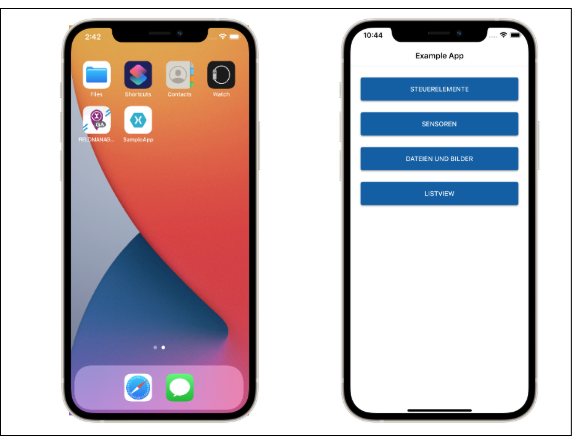
\includegraphics[width=\textwidth,keepaspectratio]{Images/Screenshot/AppIconAndMenu.png}
 \caption{Test Objekt Screenshots I}
 \label{fig:TestObjectI}
\end{figure}

Anhand des Namens,  SampleApp,  und eines Anwendungsicons können Anwender die Benutzer die App auf dem Startbildschirm identifizieren.  Nach dem Start öffnet sich eine Menüstruktur,  die Wurzel der Navigation, über die verschiedene Bereiche, der mobilen Anwendung angesteuert werden können.  In einer vertikal Ansicht werden dafür Schaltflächen als Ereignisauslöser für die Navigation bereitgestellt,  die zu den folgenden Seiten führen: Übersicht der Steuerelemente,  Ausgabe von Smartphonesensoren,  Arbeit mit Bildern und Ansicht einer Listview.   Abbildung \ref{fig:TestObjectII} zeigt die Übersicht der Steuerelemente sowie die Werte der Smartphone-Sensoren.

\begin{figure}[!ht]
 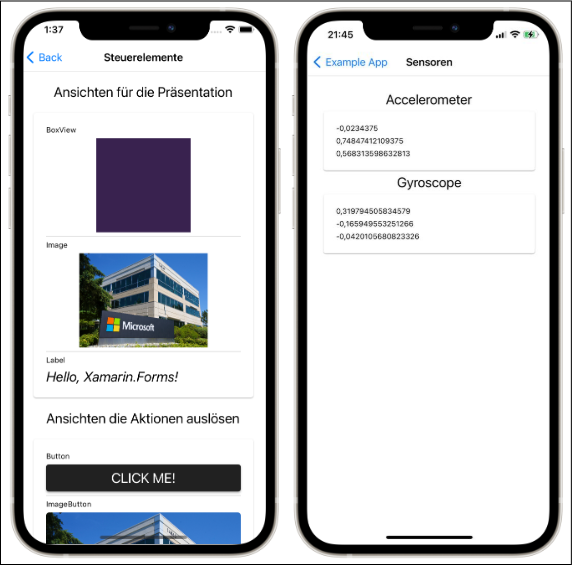
\includegraphics[width=\textwidth,keepaspectratio]{Images/Screenshot/Sensors.png}
 \caption{Test Objekt Screenshots II}
 \label{fig:TestObjectII}
\end{figure}
Die übersieht der verfügbaren Steuerelemente greift einige der häufig verwendeten Steuerelemente auf,  diese sind Anhand der in Kapitel 4 aufgeführten Kategorien gruppiert und vertikal angeordnet.  Neben dieser Darstellung ist eine Übersicht über die aktuellen Werte des Beschleunigungssensors und des Gyroskopes abgebildet,  die über das Plugin Xamarin.Essentials ausgelesen werden.  Die nächsten beiden Screenshots in \ref{fig:TestObjectIII} zeigen das Menü für die Arbeit mit Bildern und einen Berechtigungsdialog.

\newpage 
\begin{figure}[!ht]
 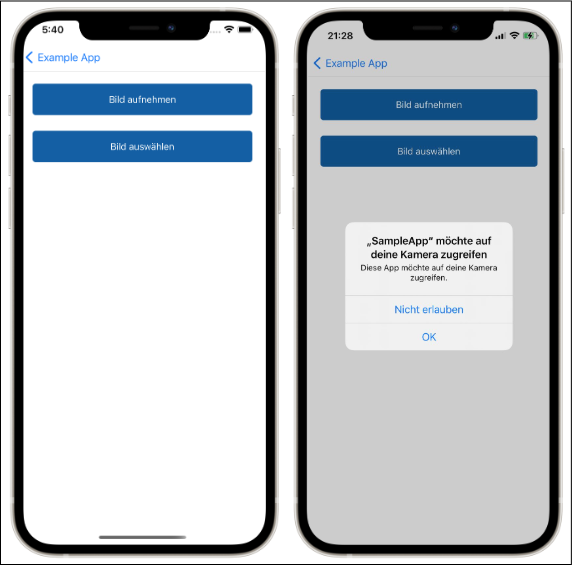
\includegraphics[width=\textwidth,keepaspectratio]{Images/Screenshot/Permissions.png}
 \caption{Test Objekt Screenshots III}
 \label{fig:TestObjectIII}
\end{figure}
Das Menü hat Ähnlichkeiten mit dem der Hauptseite,  anstatt einer Navigation werden hier jedoch plattformspezifische Funktionalitäten über das Xamarin.Essentials Plugin ausgeführt.  Diesen bieten Zugriff auf die Kamera und die Galerie des Smartphones.  Der Dialog , der nach der Zugriffsberechtigung fragt zeigt auf iOS einen Eintrag aus den Metadaten an,  der ebenfalls überführt werden muss.  
Weitere Screenshots werden in \ref{fig:TestObjectIV} gezeigt,  diese beinhalten die Auswahl eines Bildes aus der Galerie. und die Darstellung von Daten in einer ListView.  Diese stellt den Namen und die Emailadresse von  Benutzern da.  Die Klasse Benutzer wird innerhalb der des Quelltexters der mobilen Anwendung definiert.  Anschließend werden zehn Objekte dieses Typen in einer Auflistung vorgehalten und in der ListView angezeigt.
\newpage 
\begin{figure}[!ht]
 \includegraphics[width=\textwidth,keepaspectratio]{Images/Screenshot/ImagesListView.png}
 \caption{Test Objekt Screenshots IV}
 \label{fig:TestObjectIV}
\end{figure}


\section{Testfälle}
Zur Überprüfung der Funktionalität des Compilers müssen Testfälle definiert werden. Damit ist zu 
kontrollieren, ob die Übersetzung der in \Csharp{} programmierten  Xamarin.Forms Testapp eine in 
visuell und logisch vergleichbare Flutter Zielapp ergibt.  Tabelle \ref{tab:Testapp} beschreibt die Testfälle und ihre entsprechenden Funktionen.


\begin{xltabular}{\textwidth}{l|l|X}
   \textbf{ID} & \textbf{Komponente} & \textbf{Beschreibung}  \\  


\hline
1             & App-Icon           	& Prüfen ob das App-Icon übernommen wurde                      			 \\ 
2             & App-Name          	& Prüfen ob das App-Name übernommen wurde                      		 \\ 
3             & SDK Versionen      & Prüfen ob die SDK Versionen übernommen wurden                      \\ 
4             & Seitenname           				& In der Navigationsleiste wird der Name der aktuellen Seite angezeigt               \\ 
5          	  & Navigation         			  	& Mit Hilfe des Menüs kann navigiert werden                      			 \\ 
6             & Zurück Navigation           	& Über die Navigationsleiste kann zurrück Navigiert werden                      			 \\ 
7             & Gyroscope auswerten           	& Die Werte werden in der App angezeigt.                      			 \\ 
8             & Accelerometer auswerten           	& Die Werte werden in der App angezeigt.                   			 \\ 
9             & Compass auswerten           	& Die Werte werden in der App angezeigt.                			 \\ 
10            & Magnetometer auswerten           	& Die Werte werden in der App angezeigt.                			 \\ 
11            & Sensor nicht verfügbar         	& Wenn ein Sensor nicht verfügbar ist, wird ein Fehler angezeigt          			 \\ 
12            & Steuerelemente 	           		& Alle Steuerelemente werden angezeigt        			 \\ 
13            & Ereignisse funktionieren           	&  Steuerelemente reagieren wie gewohnt     			 \\ 
14            & Bild aus Ressourcen laden           	& Ein Bild aus den Ressourcen wird in der App angezeigt                   			 \\ 
15             & Bild aus dem Web laden           	& Ein Bild aus dem Internet wird in der App                      			 \\ 

	  \caption{Testfälle der Testapp}

 \label{tab:Testapp}
\end{xltabular}


\section{Testablauf}
In diesem Abschnitt werden die definierten Testfälle manuell durchgeführt und das Ergebnis dokumentiert. 
Der Start  des Testlaufs beginnt mit dem Aufruf der grafischen Benutzeroberfläche,   der Auswahl der Xamarin.Forms Testapp und eines leeren Ordners, der als Zielverzeichnis nach der Kompilierung dient. 
Aufgrund der vielen Dateizugriffe und durchzuführenden Aktionen nimmt die Übersetzung der Anwendung eine gewisse Zeit in Anspruch. Im Frontend lassen sich Informationen über den Status, den Verlauf und mögliche Fehlerquellen nach der Übersetzung ablesen.  Anschließend kann die fertige Flutter Anwendung mithilfe der SDK kompiliert und ihre Ansichten kontrolliert werden.  Die im folgenden visualisierten Screenshots zeigen die generierte iOS Flutter-App,  die entsprechenden Androidrepräsenationen befinden Anhang dieser Arbeit.  Zur Förderung der Vergleichbarkeit werden die gleichen Inhalte der mobilen Anwendung abgebildet.  In Abbildung \ref{fig:FlutterAppI} wird das Icon und der Name der Anwendung auf dem Smartphone und das zentrale Menü der App dargestellt.
\newpage
\begin{figure}[!ht]
 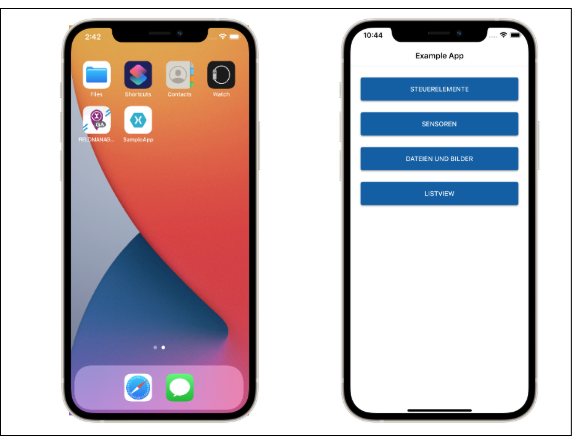
\includegraphics[width=\textwidth,keepaspectratio]{Images/Screenshot/AppIconAndMenu.png}
 \caption{Flutter App Screenshots I}
 \label{fig:FlutterAppI}
\end{figure}

Die Screenshots zeigen,  auf den ersten Blick die erwartete visuelle Vergleichbarkeit der Anwendungen.  Sowohl der Name als auch das Launchericon der Anwendung sind korrekt übernommen worden.  Nach dem Start der Anwendung fallen jedoch Designabweichungen auf, die durch die Verwendung der Material Design Vorlagen in Flutter begründet sind. Da der Compiler nicht,  wie in den Ausschlusskriterien festgelegt, den Style der Anwendung übersetzt,  entspricht das Ergebnis der Erwartungshaltung und ist, wenn daraus keine funktionellen Störungen 
entstehen,  an dieser Stelle akzeptabel.  Das zentrale Menü mit seiner Navigationsfunktion entspricht in der Ziel- dem der Testapp,  
unterscheidet sich allerdings in der Animation. Abbildung \ref{fig:FlutterAppII} zeigt die Übersicht der Steuerelemente sowie die Werte der Smartphone-Sensoren.

\newpage
\begin{figure}[!ht]
 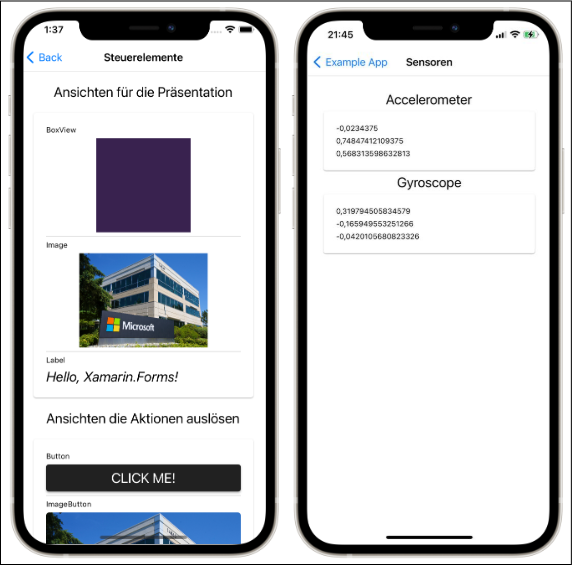
\includegraphics[width=\textwidth,keepaspectratio]{Images/Screenshot/Sensors.png}
 \caption{Flutter App Screenshots II}
 \label{fig:FlutterAppII}
\end{figure}
Die übersetzten Übersicht der Steuerelemente stimmt  bezüglich der Verschachtlungen als auch der Funktionalitäten mit denen der Xamarin.Forms Variante überein,  was beispielsweise beim Öffnen der Datum- und Uhrzeitenauswahl erkennbar ist. Ebenfalls korrekt übernommen wurde die Oberfläche der Sensorenansicht und alle Werte der Smartphonesensoren befinden sich im richtigen Format. Im Gegensatz zu Xamarin.Forms werden diese Daten jedoch nicht im gleichen Zyklus aktualisiert.  Dieser Unterschied basiert auf den Implementationen des jeweiligen Plugins und entsteht nicht durch den Übersetzer.  In der Xamarin.Forms App würden die Werte über Databindings geladen und mithilfe der INotifyPropertyChanged Schnittstelle wurde die Benutzeroberfläche im Falle von Änderungen aktualisiert.  Die Schnittstelle wurde in der Flutter Anwendung entfernt und die Stellen des Quelltextes, die Änderungen am UI vornehmen mit einem Setstate-Block umschlossen damit sich die Oberfläche aktualissiert.  Die nächsten beiden Screenshots in Abbildung \ref{fig:FlutterAppIII} zeigen das Menü für die Arbeit mit Bildern und einen Berechtigungsdialog für die Verwendung der Kamera.


 \newpage 
\begin{figure}[!ht]
 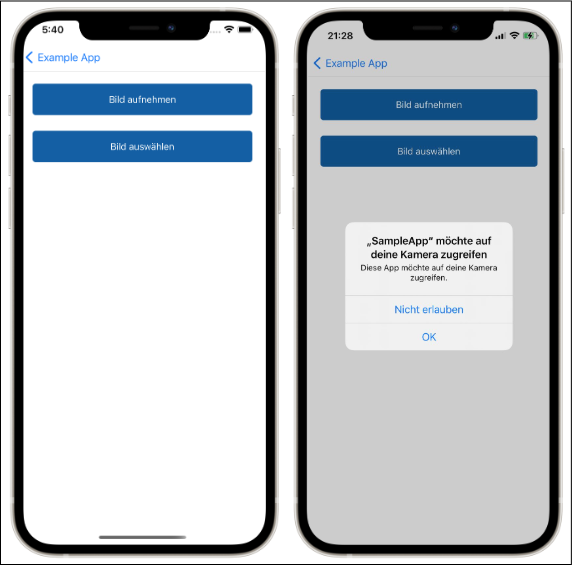
\includegraphics[width=\textwidth,keepaspectratio]{Images/Screenshot/Permissions.png}
 \caption{Flutter App Screenshots III}
 \label{fig:FlutterAppIII}
\end{figure}
Auf diesen Screenshots ist ersichtlich,  dass auch die Berechtigungen übernommen wurden,  und die Beantragung dieser genau wie bei Xamarin.Forms funktioniert.  Auch erfolgreich übersetzt wurden der Zugriff auf die Kamera und die Galerie,  mithilfe einer Erweiterung.  Dieses funktioniert wie in der ursprünglichen Version des Testobjekts.  Die letzten Screenshots darstellt in Abbildung \ref{fig:TestObjectIV} zeigen,  die Auswahl eines Bildes aus der Galerie und die Darstellung der Benutzerdaten in einer ListView.  Aus der korrekten Darstellung der ListView wird ersichtlich,  dass auch die Klassendefinition und ihr Konstruktor korrekt übersetzt wurden um die Liste mit Daten zu füllen. 
 
 \newpage 
\begin{figure}[!ht]
 \includegraphics[width=\textwidth,keepaspectratio]{Images/Screenshot/ImagesListView.png}
 \caption{Flutter App Screenshots IV}
 \label{fig:FlutterAppIV}
\end{figure}

 
Mit der im März 2021 veröffentlichten Version 2.0  können Flutter Anwendungen zu Web-Anwendungen kompiliert werden.  Auch wenn die Erstellungen von Webseiten nicht im Fokus dieser Arbeit steht soll diese Anwendung trotzdem kurz betrachtet werden.  Die grundlegende Darstellung ist identisch wie die der mobilen Anwendung.  Da das Xamarin.Forms Testobjekt jedoch nicht als Webseite ausgeführt werden kann,  ist sie nicht darauf ausgelegt auf großen Monitoren dargestellt zu werden.   Daraus folgt,  dass die Flutter App nicht für die Darstellung im Web optimiert aber lauffähig ist.  Durch die erst vor kurzem hinzugefügten Support der Webplattform haben sind noch nicht alle Erweiterung für die neue Plattform aktualisiert worden.  So ist die Funktionalität Sensor-Plugins nicht im Web verfügbar,  auch wann das Gerät über entsprechende Sensoren verfügt.  Auch das Plugin für die Verwendung der Kamera und den Zugriff auf die Bildergalerie sind nicht primär für die Verwendung im Web Entwickelt worden,  bietet jedoch die Möglichkeit Bilder hochzuladen.  Abbildung \ref{fig:WebView} zeigt einen Screenshot der Webanwendung.
\newpage
\begin{figure}[!ht]
 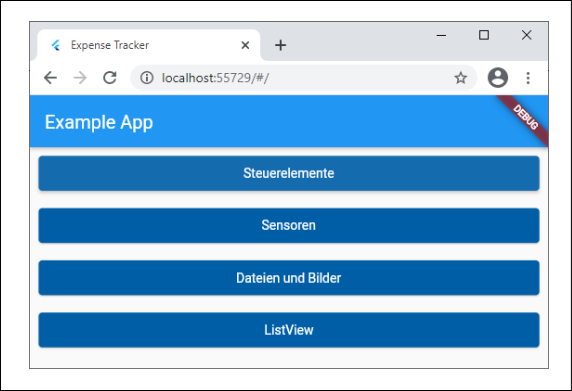
\includegraphics[width=\textwidth,keepaspectratio]{Images/Implementation/WebApp.png}
 \caption{Flutter Web-App Screenshot}
 \label{fig:WebView}
\end{figure}


Das Testobjekt konnte vollständig überführt werden, was grundsätzlich die 
Funktionsfähigkeit die Prototypen beweist. Bei einer Übersetzung aller in der Praxis möglichen 
Funktionalitäten von Xamerin.Forms bedarf es vielfältiger Erweiterungen des Compilers.


